\documentclass[article,A4,12pt]{llncs}
\usepackage[T1]{fontenc}
\usepackage{amsmath}
\usepackage{amssymb}
\usepackage{amsfonts}
\usepackage{mathrsfs, bm}

\usepackage{graphicx}
\usepackage{tabularx}
\usepackage{subfig}
\usepackage{epsf,times}
\usepackage{color}
\usepackage{wrapfig}
\usepackage{cases}
\usepackage{multicol}

\usepackage[T1]{fontenc}
%\newcommand{\tmname}[1]{\textsc{#1}}
%\newcommand{\tmop}[1]{\ensuremath{\operatorname{#1}}}
%\newcommand{\tmsamp}[1]{\textsf{#1}}
%\newcommand{\tmtextsc}[1]{{\scshape{#1}}}
%\newcommand{\tmtextsl}[1]{{\slshape{#1}}}
%\newcommand{\tmtexttt}[1]{{\ttfamily{#1}}}

\leftmargin=0.0cm
\oddsidemargin=0.5cm
\evensidemargin=0.5cm
\topmargin=0cm
\textwidth=16.0cm
%\textheight=21.5cm
\textheight=20.0cm
\pagestyle{plain}
\setlength{\columnsep}{20pt}

\def\m{\mathbf{m}}
\def\H{\mathbf{H}}
\def\E{\mathbf{E}}
\newcommand{\vepsi}{{\varepsilon}}
\def\hnorm#1#2{\vert\,#1\,\vert_{#2}}
\newcommand{\R}{{\mathbb R}}
\newcommand{\Sph}{{\mathbb S}}
\def\x{\mathbf{x}}
\def\hvec{\overline{\mathbf{h}}}
\def\evec{\overline{\mathbf{e}}}

\newcommand{ \etal}{\mbox{\emph{et al. }}}

\newcommand\vect[1]{\mbf{#1}}
\newcommand{\mbf}[1]{\mbox{\boldmath$#1$}} 
\newcommand{\RC}[1]{#1 $\times$ #1 $\times$ #1}
\def\um{$\mu$m}
\def\C{$^{\circ}\mathrm{C}$}

\newcommand{\Rmnum}[1]{\expandafter\@slowromancap\romannumeral #1@}

% DEFINITION OF CUSTOM FONT SIZE
\newcommand{\customfontA}{\fontsize{50}{55}\selectfont}
\newcommand{\customfontB}{\fontsize{14.4}{20}\selectfont}
\newcommand{\customfontC}{\fontsize{30}{35}\selectfont}

\DeclareMathAlphabet{\mathpzc}{OT1}{pzc}{m}{it}

\def\clovek#1{\noindent\bgroup\vbox{\noindent#1}\egroup\vskip1em}



\begin{document}



%%%%%%%%%%%%%%%%%%%%%%%%%%%%%%%%%%%%%%%%%%%%%%%%%%%%%%%%%%%%%%%%%%%%%%%%%

\pagestyle{empty}
\vbox{}

\pagestyle{empty}

%\begin{figure}[!ht]
%\begin{center}
%
\includegraphics[width=\textwidth]{img/NCLab-Programming-1.png}
%\end{center}
%\end{figure}
\vbox{}
\vspace{2cm}

\begin{center}
{\huge \bf First Course in Programming}
\end{center}

\begin{figure}[!ht]
\begin{center}
\vspace{-6mm}
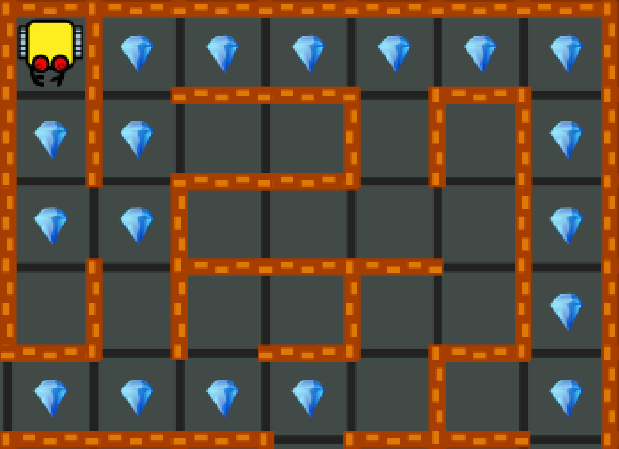
\includegraphics[width=0.26\textheight]{imgk/karel-logo.png}\ \ \ \ \ \ 

\includegraphics[width=0.2\textheight]{imgp/python-logo.png}
\vbox{}
\vspace{-9mm}
\end{center}
\end{figure}
\begin{center}
{\huge \bf with Karel the Robot and Python}
\end{center}
\vbox{}
\vspace{3cm}
\centerline{\Large \bf Solution Manual}
\begin{center}
\vfill
{\large
{\bf Pavel Solin}, University of Nevada, Reno\\
{\bf Salih Dede}, Coral Academy of Science, Reno
}
\end{center}
\newpage
\vbox{}
\vfill
\begin{center}
{\large
This solution manual is part of the online course 
{\em Intro to Programming with Karel the Robot and Python} 
({\tt http://introtoprogramming.net}) and its use is allowed 
with current subscription only. Distribution or sharing is not allowed. \\
}
\vfill

Copyright 2012 FEMhub Inc. All rights reserved.
\end{center}




\section*{}
\small

\normalsize

\newpage
%{\ }
\setcounter{tocdepth}{2}
\tableofcontents
%\pagestyle{plain}

\newpage

\pagestyle{plain}
\setcounter{page}{1}

%%%%%%%%%%%%%%%%%%%%%%%%%%%%%%%%%%%%%%%%%%%%%%%%%%%%%%%%%%%%%%%%%%%%%%%%%

\section{Solutions to Tutorial Games}

This Solution Manual provides solutions to all exercises in the 
Programming mode of the tutorial "First Course in Programming with
Karel the Robot", as well as to some other games. All programs shown 
in the following are also available through the File Manager's Project 
$\rightarrow$ Clone menu.


\subsection{B01 - Go Command}
\begin{verbatim}
go
go
\end{verbatim}

\subsection{B02 - Get Command}
\begin{verbatim}
go
get
go
get
go
get 
go
\end{verbatim}



\subsection{B03 - Left and Right Commands}
\begin{verbatim}
left
go
left
go
get
right
go
left
go
\end{verbatim}



\subsection{B04 - Put Command}
\begin{verbatim}
go
get
left
left
go
go
put
left
left
go
left 
go
\end{verbatim}


\subsection{C01 - Sprint}
\begin{verbatim}
repeat 10
  go
\end{verbatim}

\subsection{C02 - Lucky Strike}
\begin{verbatim}
left
repeat 5
  go
repeat 12
  get
left
repeat 5
  go
\end{verbatim}

\subsection{C02 - Feelin' Lucky}
\begin{verbatim}
go
repeat 20
  left
repeat 3 
  go
get
repeat 2
  left
repeat 4
  go
\end{verbatim}

\subsection{C02 - Garage Sale}
\begin{verbatim}
go
repeat 10
  put
repeat 2
  left
go
\end{verbatim}

\subsection{C05 - String of Gems}
\begin{verbatim}
repeat 10
  go
  get
\end{verbatim}

\subsection{D01 - In the Fog}
\begin{verbatim}
repeat 10
  if gem
    get
  go
\end{verbatim}

\subsection{D02 - Stony Meadows}
\begin{verbatim}
repeat 14
  if gem
    get
  if not wall
    # you can go:
    go
  else
    # avoid the stone:
    left
    go
    repeat 2
      right
      go
    left
\end{verbatim}

\subsection{D03 - Filling the Blanks}
\begin{verbatim}
repeat 11
  go
  left
  go
  if not gem
    put
  repeat 2
    left
  go
  left
\end{verbatim}


\subsection{E01 - South West}
\begin{verbatim}
# orient the robot to face north:
while not north
  left
# now turn him to face south:
repeat 2
  left
# go to the south border of maze:
while not wall
  go
# turn right:
right
# walk straight home:
while not home
  go
\end{verbatim}

\subsection{E02 - Hide-and-Seek}
\begin{verbatim}
while not home
  if not wall
    go
  if gem
    left
    get
\end{verbatim}

\subsection{E03 - Walk the Line}
\begin{verbatim}
# align the robot with the wall:
while not wall
  left
right

while not home
  go
  left
  if not wall
    # we are at the end
    go
    left
  else
    # not the end yet
    right
\end{verbatim}

\subsection{F01 - Four Star Hotel}
\begin{verbatim}
# Shortcut for three commands:
def gogetgo
  go
  get
  go

# PIck one star:
def getstar
  repeat 2
    go
  repeat 4
    gogetgo
    left
  go
  left
  gogetgo

# Main program:
repeat 3
  getstar
  go
  right
getstar
right
repeat 3
  go
\end{verbatim}

\subsection{F02 - U-Haul}
\begin{verbatim}
# Define function to either
# get or put a gem:
def try
  if gem
    get
  else
    if not empty
      put

# Do this for one column:
def column
  repeat 5
    try 
    go
  try
      
# Define function to 
# traverse the square:
def traverse
  repeat 3
    column
    right
    go
    right
    column
    left
    # Only used for the 
    # putting part:
    if not wall
      go 
      left

# Get there:
left
repeat 6
  go
   
# Collect gems:
traverse

# Move to the lower 
# left corner:
repeat 2
  left
while not wall
  go
left
repeat 3
  go
left

# Put the gems:
traverse

# Get homw:
repeat 2
  left
while not home
  go
\end{verbatim}

\subsection{F03 - Egg Hunt}
\begin{verbatim}
# Get all gems in pile:
def getall
  while gem
    get

# Move forward one step
# and get gem if any:
def move
  go
  getall
    
# Move 2 times:
def move2
  repeat 2
    move
    
# Move 3 times:
def move3
  repeat 3
    move

# Move 4 times:
def move4
  repeat 4
    move

# Search one cell (assumes
# that Karel stands in front
# of the entrance):
def onecell
  move
  right
  move2
  left
  move3
  left
  move4
  left
  move3
  left
  move
  left
  move2
  right
  move2
  right
  move
  right
  move
  left
  move2

# Go to the next cell:
def gotonext
  left
  repeat 5
    go
  left
  
# Search three cells:
def searchthree
  repeat 2
    onecell
    gotonext
  onecell
  
# Go to the first cell:
move2
left
move2

# Search top cells:
searchthree

# Move across:
move3

# Search bottom cells:
searchthree

# Return home:
go
left
repeat 2
  go
\end{verbatim}

\subsection{F04 - Blind Carpenter}
\begin{verbatim}
# Find nearest corner:
def find_corner
  left
  while wall
    right
    if not home
      go
      left
    
# Find out whether the opening
# in front of you is a window
# slot of the corner of the house. 
def check_window
  if not home
    go
    right
    if wall
      put
      right
      go
      left
      go
    else
      left
    
# Main program:
while not home
  find_corner
  check_window
\end{verbatim}


\subsection{F05 - Pirate Ship}
\begin{verbatim}
# The three commands below are 
# elementary and you should be
# defining them as the last thing.
# Read this code from below. 
# Long step.
def longstep
  repeat 2
    go

# Version of longstep where Karel
# may get home.
def longstephome
  go
  if not home 
    go
    
# Turn back.
def turnback
  repeat 2
    left

# Get pair of gems that lie across 
# the aisle, and move to next pair.
# This should be your third part
# of code to write.
def gettwo
  go
  left
  go
  get
  turnback
  longstep
  get
  turnback
  go
  right

# Empty an entire aisle and 
# get ready for the next one.
# This should be your second 
# part of the code to write.
def emptyaisle
  go
  right
  while not wall
    gettwo
  turnback
  while not wall
    go
  right
  longstephome
    
# Karel does not know how many 
# aisles there are, so he will 
# be emptying them until he 
# gets home. This should be your
# first part of code to write.
while not home
  emptyaisle
\end{verbatim}

\subsection{F06 - Diamond Staircase}

\begin{verbatim}
def onestep
  left
  go
  right
  go 
  get
  
while not home
  onestep
\end{verbatim}

\subsection{F07 - Plucking Flowers}

\begin{verbatim}
repeat 4
  repeat 7
    go
    get
  left
\end{verbatim}

\subsection{F08 - Gems for Friends}

\begin{verbatim}
# go four steps forward:
def foursteps
  repeat 4
    go

repeat 4
  # go to the middle:
  foursteps
  # turn to the left:
  left
  # enter friend's house:
  foursteps
  # put a gem on the ground:
  put
  # turn back:
  repeat 2
    left
\end{verbatim}

\subsection{F09 - Diamond Rectangle}

\begin{verbatim}
go
while not home
  while gem
    # collect all gems in the pile:
    while gem
      get
    # move on one step:
    go
  # we reached the end - turn 
  # only if not home yet:
  if not home
    repeat 2
      left
    go
    right
    go
\end{verbatim}

\subsection{F10 - Gem Jam}

\begin{verbatim}
while not home
  while not wall
    if gem
      get
    go
  left
\end{verbatim}

\subsection{F11 - The Matrix}

\begin{verbatim}
# Pick up 15 gems:
def get15
  if gem
    get
  repeat 14
    go
    if gem
      get
      
# Pick up 11 gems:
def get11
  if gem
    get
  repeat 10
    go
    if gem
      get
      
# Left turn:
def leftturn
  left
  go
  if gem 
    get
  go
  left
  
# Right turn:
def rightturn
  right
  go
  if gem 
    get
  go
  right

# Clear two columns:
def clear2columns
  get11
  leftturn
  get11
  rightturn

# Clear two rows:
def clear2rows
  get15
  leftturn
  get15
  rightturn
  
# Get to initial position:     
right
go

# First clear all vertical aisles:
repeat 3
  clear2columns
get11
leftturn
get11

# Get in position to clear horizontal
# aisles:
left

# Clear all horizontal aisles:
repeat 2
  clear2rows
get15
leftturn
get15

# Get ready to return home:
left

# Go home:
while not home
  go
\end{verbatim}

\subsection{F12 - Escape from Alcatraz}

\begin{verbatim}
# Align the robot so that wall is 
# on its right.
def align_with_wall
  while not wall 
    left
  left

# Make a step along the wall (and 
# around a corner if needed). Assumes 
# that wall is on your right. 
def step_along_wall
  while wall 
    left
  go
  # Check whether there is a corner.
  right
  if wall 
    left   # No corner.   
  else     # Corner.
    go
    right
    if wall 
      left
    else 
      go
      
# Step along the wall until you reach 
# home. Assumes that Karel stands next 
# to a wall that is connected to an 
# exterior wall.
def search_tunnels
  align_with_wall
  while not home
    step_along_wall

while not wall
  go
search_tunnels
\end{verbatim}

\subsection{F13 - Border Patrol}

\begin{verbatim}
# Align the robot so that wall is 
# on its right.
def align_with_wall
  while not wall 
    left
  left

# Make a step along the wall (and 
# around a corner if needed). Assumes 
# that wall is on your right. 
def step_along_wall
  while wall 
    left
  go
  if gem 
    get
  # Check whether there is a corner.
  right
  if wall 
    left   # No corner.   
  else     # Corner.
    go
    if gem 
      get
    right
    if wall 
      left
    else 
      go
      if gem 
        get

# Step along the wall until you reach 
# home. Assumes that Karel stands next 
# to a wall that is connected to an 
# exterior wall.
def border_patrol
  align_with_wall
  while not home
    step_along_wall

border_patrol
\end{verbatim}

\subsection{F14 - Ariadne's Thread}

\begin{verbatim}
# Turn back:
def back
  repeat 2
    left

# Program assumes that Karel faces the last gem.
# The chain of gems should not have loops.
def get_next_gem
  if not wall
    if not home
      go
      if gem 
        get
      else
        if not home
          back
          go
          left
          if not wall
            if not home
              go
              if gem 
                get
              else
                if not home
                  back
                  repeat 2 
                    go
                  get
          else
            if not home
              back
              go
              get
  else 
    left
    if not wall
      if not home
        go
        if gem 
          get
        else
          if not home
            back
            repeat 2 
              go
            get
    else
      if not home
        back
        go
        get

def ariadnes_thread
  while not home
    get_next_gem
        
ariadnes_thread
\end{verbatim}

\subsection{G01 - Cheese!}

\begin{verbatim}
def peel_edge
  go
  while gem
    get
    go
  repeat 3
    right
    go
  go
  if gem
    get
    peel_edge
      
# Eat the cheese:
peel_edge

# Return home:
while not north
  left
while not wall
go
left
while not home
  go
\end{verbatim}

\subsection{G02 - Speleologist}

\begin{verbatim}
# Descend one step, explore the rest,
# and return:
def explore
  if not wall
    go
    right
    if not wall
      go
      left
      explore
      right
      go
      left
      go
    else
      right
      go
  else 
    repeat 2
      left
      go
    
# Explore cave and return home:
explore
while not home
  go
\end{verbatim}

\subsection{G03 - Homage to Lemmings}

\begin{verbatim}
# Turn back.
def back
  repeat 2
    left
  
# Add layer of gems, return, and
# get ready for next layer.
def addlayer
  if not home
    while not wall 
      go
      put
    # Turn back and return.
    back
    while gem
      go
    back
    # Get ready for next layer.
    go
    left
    go 
    right
    addlayer
    
addlayer
\end{verbatim}

\subsection{G04 - Diamond Tree}

\begin{verbatim}
# Turn back.
def back
  repeat 2
    left

# Right angle.
def rangle
  go
  right
  go
  
# Left angle.
def langle
  go
  left
  go
  
# Return from left branch to base.
def return_from_left_branch
  right
  rangle
  back
  
# Return from right branch to base.
def return_from_right_branch
  left
  langle
  back
  
# Robot faces left wall after 
# an attempt to find new branch 
# on the left.
def return_from_left_wall
  left
  go
  back
  
# Robot faces right wall after
# an attempt to find new branch 
# on the right.
def return_from_right_wall
  right
  go
  back
  
# Assumes that Karel stands on a gem.
def left_branch
  # Is there a wall in the North?
  if not wall
    go
    left
    # Is there a wall in the West?
    if not wall
      go
      right
      if gem
        climb_tree
      return_from_left_branch
    else
      return_from_left_wall

# Assumes that Karel stands on a gem.
def right_branch
  # Is there a wall in the North?
  if not wall
    go
    right
    # Is there a wall in the East?
    if not wall
      go
      left
      if gem
        climb_tree
      return_from_right_branch
    else
      return_from_right_wall

# Traverse recursively first the 
# left and then the right branch.
# Then pick up the base gem.
def climb_tree
  left_branch
  right_branch
  if gem
    get

# Move to tree.    
go
# Traverse it recursively.
climb_tree
# Go home.
right
rangle
\end{verbatim}

\subsection{H01 - Accounting}

\begin{verbatim}
def accounting
  num = zero
  while not empty
    put
    inc(num)
  return num

n = accounting
print "I have", n, "gems in the bag."
\end{verbatim}


\subsection{H02 - Tape Measure}

\begin{verbatim}
def measure
  # Go to the west wall
  # and turn east:
  while not north
    left
  left
  while not wall
    go
  repeat 2
    left
  # Start measuring:
  len = zero
  while not wall
    inc(len)
    go
  return len
  
l = measure
print "Width of the room is", l
\end{verbatim}


\subsection{H03 - Orchard}

\begin{verbatim}
def orchard
  num = zero
  repeat 6
    # Check the tile you stand on:
    while gem
      inc(num)
    # Check the rest of the row:
    while not wall
      go
      while gem
        inc(num)
    # Move to next row and turn back:
    left
    if not wall
      go
    left
    # Check the tile you stand on:
    while gem
      inc(num)
    # Check the rest of the row:
    while not wall
      go
      while gem
        inc(num)
    # Move to next row and turn back:
    right
    if not wall
      go
    right

n = orchard
print "There are", n, "apples in the orchard."
\end{verbatim}


\subsection{H04 - New Carpet}

\begin{verbatim}
# Count tiles in one row. Assumes
# that Karel stands at the West end 
# of the row, facing East: 
def check_row
  n = 1
  while not wall
    go 
    inc(n)
  return n
  
# Assumes that Karel is at the 
# East end of a row, facing East:
def one_row_up
  finished = False
  left
  while wall
    left
    if not wall 
      go
    else 
      finished = True 
    right
  go
  return finished

# Move to the West end of row 
# and turn East. Assumes that 
# Karel faces North:
def get_west
  left
  while not wall
    go
  repeat 2
    left
  
# Measure the area:
def carpet
  a = check_row
  while one_row_up
    get_west
    inc(a, check_row)
  return a
  
# Calculate and print apartment area:
area = carpet
print "Carpet size =", area
\end{verbatim}


\subsection{I01 - Reading Numbers}

\begin{verbatim}
# Make two steps:
def go2
  repeat 2 
    go

# Read number in box:
def readnumber
  # First detect gems
  # at key positions:
  go
  gem10 = gem
  go2
  gem12 = gem
  go2
  gem14 = gem
  right
  go
  right
  go
  gem23 = gem
  right
  go2
  gem03 = gem
  left
  go2
  gem01 = gem
  left
  go
  right
  go2
  repeat 2
    left
  
  # Decide what number is in 
  # the box:
  if gem10
    # 0, 2, 4, 5, 6, 8:
    if gem12
      # 2, 3, 5, 6, 8:
      if gem03
        # 5, 6, 8:
        if gem23
          # 4:
          return 4
        else
          # 5, 6:
          if gem01
            # 6:
            return 6
          else 
            # 5:
            return 5
    else
      # 0:
      return 0
  else
    # 1, 4, 7:
    if gem12
      # 4:
      return 4
    else
      # 1,7:
      if gem14
        # 7:
        return 7
      else
        # 1:
        return 1

# Main program:
n1 = readnumber
print "Number in the first box is", n1

# Move to second box:
right
repeat 3
  go
left

n2 = readnumber
print "Number in the second box is", n2

# Move to third box:
right
repeat 3
  go
left

n3 = readnumber
print "Number in the third box is", n3
\end{verbatim}

\subsection{I02 - Writing Numbers}

\begin{verbatim}
# Coming soon.
\end{verbatim}

\subsection{I03 - Adding Numbers}

\begin{verbatim}
# Coming soon.
\end{verbatim}

\subsection{I04 - Eight Queens}

\begin{verbatim}
# Coming soon.
\end{verbatim}

\subsection{I05 - BubbleSort}

\begin{verbatim}
# Coming soon.
\end{verbatim}


\end{document}

 
